\documentclass[11pt]{article}

\usepackage{amssymb,amsmath,amsfonts,eurosym,geometry,ulem,graphicx,caption,color,setspace,sectsty,comment,footmisc,caption,natbib,pdflscape,subfigure,array,hyperref,epigraph,multirow,tabu}

\usepackage[T1]{fontenc}
\usepackage[utf8]{inputenc}
\usepackage{tgpagella}
\usepackage{todonotes}
\usepackage{textcomp}
\usepackage{eurosym}
\usepackage{hyperref}
\usepackage{tcolorbox}

\normalem

\onehalfspacing
\setlength{\parskip}{0.3em}

\newtheorem{theorem}{Theorem}
\newtheorem{corollary}[theorem]{Corollary}
\newtheorem{proposition}{Proposition}
\newenvironment{proof}[1][Proof]{\noindent\textbf{#1.} }{\ \rule{0.5em}{0.5em}}

\newtheorem{hyp}{Hypothesis}
\newtheorem{subhyp}{Hypothesis}[hyp]
\renewcommand{\thesubhyp}{\thehyp\alph{subhyp}}

\newcommand{\red}[1]{{\color{red} #1}}
\newcommand{\blue}[1]{{\color{blue} #1}}

\DeclareMathOperator*{\argmax}{arg\,max} 

\newcolumntype{L}[1]{>{\raggedright\let\newline\\arraybackslash\hspace{0pt}}m{#1}}
\newcolumntype{C}[1]{>{\centering\let\newline\\arraybackslash\hspace{0pt}}m{#1}}
\newcolumntype{R}[1]{>{\raggedleft\let\newline\\arraybackslash\hspace{0pt}}m{#1}}

\geometry{left=1.0in,right=1.0in,top=1.0in,bottom=1.0in}

\begin{document}

%+Title
\title{%
\textbf{Mapping Research \& Innovation Missions \\
\large With an application to the UK Government Mission to transform the prevention, diagnosis and treament of chronic diseases using Artificial Intelligence}}
\author{Juan Mateos-Garcia}
%\date{}
\maketitle
%-Title
%+Abstract
\begin{abstract}
Mission-oriented innovation policies to address specific technological, social or economic challenges are being increasingly recognised as a promising strategy to steer innovation in societally desirable directions and encourage the formation of new disciplines and industries. The formulation of this policy agenda has however raced ahead of the evidence base, creating the risk that mission-oriented innovation policies are insufficiently informed in their formulation, targeting, monitoring and evaluation. We argue that developing a suitable evidence base for mission-oriented policies will require the use of new data sources, analytical methods and indicators that reflect their rationale and pathways to impact through network-building and interdisciplinary crossover, and help manage the risks of capture and `picking winners' prematurely. We deploy these methods to develop prototype indicators in the empirical setting of the UK government Grand challenge to \textit{`Use data, Artificial Intelligence and innovation to transform the prevention, early diagnosis and treatment of chronic diseases by 2030`}. Having identified an `active mission field' of projects that combine AI and chronic disease-related keywords, we show that although chronic diseases are underrepresented among AI projects, this situation has started to change in recent years, with fast growth in the active mission field. We also find that projects in the active mission field tend to generate more technological outputs, combine various disciplines, and involve younger specialist organisations. We conclude with an experimental analysis of the `trajectories' of the active mission field using a hierarchical topic modelling approach, and show that topics related to AI tend to be more prevalent that topics related to chronic diseases in the active mission field, suggesting that its exploration of technological opportunities is being driven by computer scientists rather than medical scientists and biotechnologists. Having said this, the diversity of trajectories being explored in the active mission field has not decreased over time, consistent with the idea that it is not settling prematurely into a dominant `solution' for its challenge. We hypothesise that is a consequence of the diversity of funders participating in the active mission field. 
\end{abstract}
%-Abstract

\section{Introduction}
\label{sec:introduction}

Mission-oriented Research \& Innovation policies are systemic public policies that draw on frontier knowledge to attain specific goals or `big science deployed to meet big problems' (Mazzucato, 2018). Missions are at the core of new €100bn EU proposal for Horizon Europe (released June 2018), and of the new industrial strategy developed by UK government, which is organised around the idea of `Grand Challenges’ that generate missions, as well as an `Industrial Strategy Challenge Fund’ that identifies particular challenges to be pursued through concerted policy action (HM Government, 2018). Some mission ideas and policies include \textit{`Reach net zero greenhouse gas emissions balance of 100 European cities
by 2030'} (Mazzucato, 2018), or \textit{`Ensure that people can enjoy at least 5 extra healthy, independent years of life by 2035, while narrowing the gap between the experience of the richest and poorest'} (BEIS, 2018). The figure below illustrates a mission specification from Mazzucato (2018).

\begin{figure}[!ht]
    \centering
    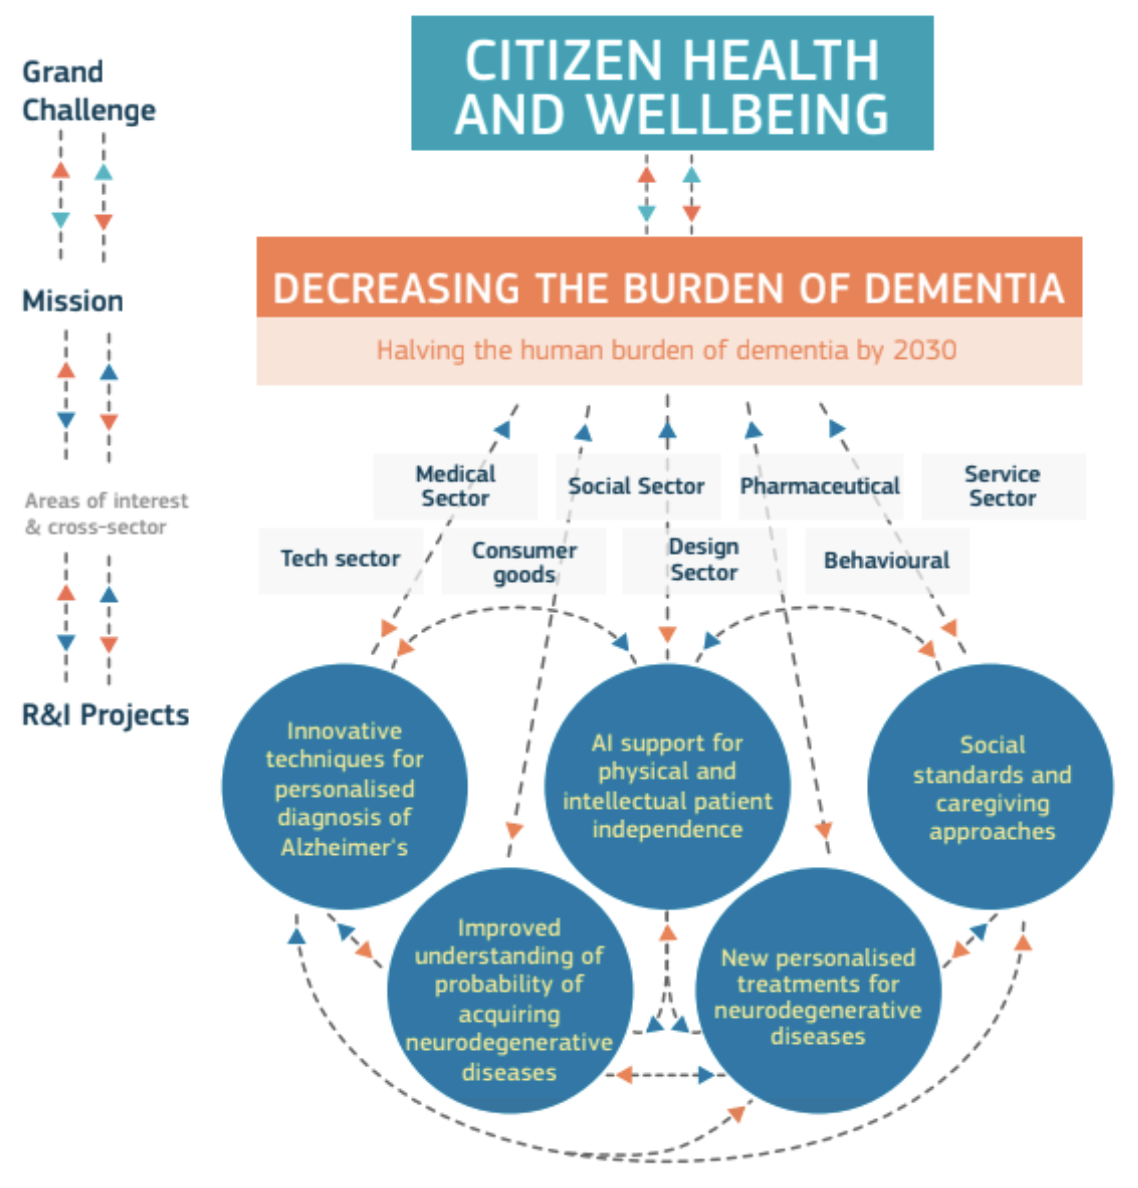
\includegraphics[width=0.5\textwidth]{figures/fig1_example.png}
    \caption{A mission example (taken from Mazzucatto (2018))}
    \label{fig:mission_example}
\end{figure}

Missions could help bridge worrying disconnects between technology development, societal well-being and productivity growth by actively encouraging the deployment of new technologies to tackle societal challenges and supporting the exploration of new technological trajectories where `new ideas are less hard to find' (\todo{add ref} Bloom etc). At the same time, missions present important risks: they could fail to target the most significant societal challenges resulting in a loss of legitimacy for their administrators and R\&I policy more widely, they may be unrealistic or unfeasible, or `pick winners' that are commercially unsustainable, rent-seeking or induce premature lock-in to weaker technologies. 

Realising the potential of missions while managing these risks requires a suitable evidence base and indicators for policy prioritisation, targeting, monitoring and evaluation. In this paper, we contribute to this evidence base by developing prototype indicators focusing on one particular mission \- the mission to transform the prevention, diagnosis and treatment of chronic diseases using `Artificial Intelligence, Data and Innovation' announced by UK Government in 2018. In doing this, we explore the potential of unstructured data and data science methods for generating relevant and inclusive indicators for R\&I policies increasingly concerned with the deployment of emerging technologies in particular directions. 

In the rest of this section, we review the literature about mission-oriented R\&I policies, highlighting their characteristics, rationales, risks and evidence needs, and outline the goals of the paper as well as our research questions. Having done this, in Section \ref{sec:methodology} we describe our methodology, including data collection, processing and enrichment activities, and the approach we have used to operationalise our focus mission in order to generate indicators about it. Section \ref{sec:findings} presents our findings and Section \ref{sec:conclusion} ends with a discussion of the implications of our analysis, its limitations and issues for further research.

\subsection{A rationale for innovation missions}
\label{subsec: history}

Missions are not new in R\&I policy. Some of humankind`s greatest technical achievements have resulted from missions. Some examples include the Longitude Reward, which encouraged the development of sea watches greatly improving the safety of sea travel in the 18th Century, the Manhattan Project to develop an atomic bomb, or the Apollo program to put a man on the moon (Mowery, Nelson, \& Martin, 2010; Nelson, 1977). Mission-like policies also play an important part in the private sector through crowdsourcing challenges and competitions (a comparative assessment of some of the biggest and most influential frameworks can be accessed \todo{add links} here). 

One thing that sets the `new wave' of missions in R\&I policy apart from previous ones is their shift away from purely technical or economic problem\-solving, and their ambition to deploy science and technology to address big social challenges that people face in their daily lives. One implicit goal of this effort is to build popular support for R\&I policies that can otherwise feel removed from everyday aspirations and concerns about the environment, health, education and inequality (Mazzucato, 2018b). This move away from technical goals to social ones creates new challenges for R\&I policy and its stakeholders, as the goal of
innovation research and policy shift from advancing knowledge and producing technical breakthroughs to achieving social changes which are harder to measure and in some cases even contested, as we see in ongoing debates about how to tackle climate change or increase social mobility (Nelson, 1977, 2011). This broader and arguably more ambitious definition of missions also requires engaging a wider set of disciplines, overcoming barriers to interdisciplinary collaboration.

Another important reason for renewed interest in the mission framework is the notion that traditional R\&I policies based on market failure and system failure rationales ignore the directionality of technical change, have low additionality and tend to be captured by the status quo (Cantner \& Vannuccini, 2018; Frenken, 2017). In other words, they support incremental activities that might not be the most societally desirable, and in some cases would have been carried out anyway, generally by powerful, established incumbents (Frenken, 2017). 

This way of thinking about the goals of R\&I policy draws on evolutionary economics and complexity science ideas suggesting that technological development is directional (it can unfold in many possible trajectories) and uncertain in outcomes. It also moves away from notions of optimality in technical change: The trajectories of development that are selected ‘from the bottom up’, for example by market forces might not be the most beneficial one if they generate unanticipated externalities and path dependences that prevent shifts away from it further down the line, as we see in the economy’s lock-in to environmentally unsustainable fossil fuels (Aghion, David, & Foray, 2009; Arthur, 2009; David, 1985). Further. ‘normal’ R\&I takes place through an exploration of the ‘adjacent possible’ where bodies of knowledge that are technically closer tend to be recombined more often because they exist in the same organisation, or in related organisations (Boschma, 2005; Hidalgo et al., 2018). All this means that R\&I policies that simply seek to increase the amounts invested in R&D (as R\&D tax credits do under a market failure rationale) or the responsiveness of academic researchers to industry needs (as knowledge exchange programs informed by a systems failure rationale do) will fail to generate societally beneficial, boundary spanning innovations (Gustafsson & Autio, 2011). 

Many recent expressions of dissatisfaction with the status quo of research and innovation policy reflect this view. Some examples include concerns about a `bubble' in biomedical research, an AI bias towards automating labour instead of complementing it, and evidence of a productivity puzzle where increasing investments on R\&D fail to produce corresponding improvements in productivity growth and societal well\-being (Acemoglu \& Restrepo, 2018; Jones & Wilsdon, 2018; Restrepo & Acemoglu, 2018; Sarewitz, 2016).

A mission-oriented R&I framework could help address these challenges: by definition, missions are directional. They identify preferred trajectories of technological development (in the examples we provided at the beginning, use of urban infrastructure and built space innovations to reduce carbon emissions, or of AI to address chronic diseases) and provide resources for pursuing them. They also encourage combinations of knowledge residing in faraway parts of the innovation system. This should yield new ideas for which there is not a market yet (otherwise they would already be deployed to address the mission) (Autio, 2011). This could involve new players sitting in the intersection between disciplines, and with a greater tolerance for risk. 

\subsection{Developing an evidence base for missions}

Innovation missions are not without risks, such as for example that R\&I policymakers without sufficient information `pick winners’ that are not feasible or commercially sustainable, that they are captured by new vested interests that coalesce around missions, or that they distort technology deployment leading to premature lock-in to weak standards and solutions (Aghion et al., 2009). Proponents of the new wave of mission-oriented policies have put in place specific criteria for mission selection and delivery to address these design and implementation challenges, ensuring that missions have legitimacy and broad social support, can be achieved, and bring together a broad mix of actors going beyond `the usual suspects'. The demand for bottom-up experimentation acknowledges uncertainty about which of the avenues that are explored through the mission will be successful, and the need to avoid picking winners that end in a technological or commercial dead-end.  

Table \ref{tab:criteria} summarizes their criteria and their implications for measurement.

(see table 1) (Mazzucato, 2018b).

\begin{table}[!]
\centering
\begin{tabu} to \textwidth {  X[l]  X[l]  X[l]  }
 \\
 \\
 \textbf{Mission selection criterion} & \textbf{Measurement question} & \textbf{Indicators}
 \\
 \hline
 \\
 \textbf{1. Social relevance:} Missions should be bold, inspirational and with wide societal relevance & 
 Is the mission societally relevant?
 \newline
 \newline Are the public and civic society engaged with the mission?

 & Measures of prevalence of the societal challenge that the mission seeks to address
 \newline
 \newline Expressions of societal need around the mission in public and media discourse
 \\
 \\
 \textbf{2. Feasible distinctiveness}: Ambitious but realistic R\&I activities
 & Do the activities supported by the mission draw on but are qualitatively different from previous research?
 \newline
 \newline What is the technological readiness of mission-related activities?
 
 & Distinctiveness/relatedness between mission activities and the status quo
 
 \newline Applied outputs from mission-related activity
 
 \\
 \\
 \textbf{3. Induces crossover:} Cross-disciplinary, cross-sectoral, and cross-actor
 & Is the mission encouraging new combinations of disciplines, technologies and industries? 
 \newline
 \newline
 Is the mission attracting new actors into the Research \& Innovation system?
 
 & Disciplinary diversity and novelty of participants compared to the status quo.
 \\
 \\
 \textbf{4. Diverse solutions:} Multiple, bottom-up solutions.
 & Is the mission enabling diversity and experimentation with multiple alternative and potentially complementary approaches to tackle its challenge?
 & Diversity of activities being supported
 \\
 \\
 \textbf{5. Measured clear direction:} measurable, time-bound 
 
 & Are the R\&I activities taking place as part of the mission achieving its goals?
 
 & Design features of the mission (KPIs, duration)
 \newline 
 \newline Attribution of impacts to mission activities
 
 \\
 \\
 \hline
\end{tabu}
\caption{Mission goals, measurements and indicators, based on (cite Mazzucatto)}
\label{tab:criteria}
\end{table}

What does this mean for the evidence base for innovation missions?

First, an evidence base for missions should capture the extent to which the topic of a mission reflects societal interests and concerns, as well as the levels of social engagement with the mission topic, and with the mission itself. It is possible to generate indicators capturing the social relevance dimension of missions with data from opinion surveys, policy debates, news media and social media, as well as indicators about the severity and prevalence of the challenge that the mission seeks to address.

Second, the evidence base needs to consider the content of the R\&I activities taking place as part of the mission, and how they balance feasibility (the activities taking place need to be technologically plausible and possible) and ambition (the activities would not have taken place without the mission). This can be measured with indicators reflecting the similarity (or differences) between R&I activities taking place as part of the mission and previous work, as well as the extent to which the projects taking place inside the mission
generate technological outputs (i.e. are technologically feasible).

Third, it is also important to consider the diversity of activities that are being supported through the mission in terms of the disciplines, industries and actors involved: are these novel and unexpected, and do they involve new `entrants’? Here we can develop indicators measuring the disciplinary and industry mix of the activities supported by a mission, and compare the actors participating in it with those involved in areas outside of the mission. Over time, we would expect successful missions to change the structure of R&I networks, bringing key disciplines and the actors involved in them into new fields and communities. We should develop indicators that capture this.

Finally, the evidence base should capture the time\-lines and goals of the mission: what does it seek to achieve, over what period, and with what success. Some of the relevant indicators can be directly extracted from the specification of the mission (eg reach zero greenhouse emissions by 2030). This is a different question from whether these indicators are being measured in a suitable way, and from the extent to which changes in those indicators (impacts) can be attributed to the mission itself (as compared to broader socio-economic trends and technological breakthroughs supported outside of the mission). 

\subsection{About this paper}
\label{subsec: about}

In this paper we develop and explore prototype indicators operationalising key dimensions of the evidence base for missions outlined above. We do this in the context of the UK Grand Challenge Mission to \textit{`Use data, Artificial Intelligence and innovation to transform the prevention, early diagnosis and treatment of chronic diseases by 2030'}, and using data about research grant funding in the UK from the Gateway to Research open dataset. Our goal is to develop a flexible framework that can be used to query funding data and identify a `mission field'. 

We define a mission field as the set of R&I activities that are directly relevant for a mission. We establish relevance using a semantic approach that extracts keywords from the definition of a mission and then queries the funding corpus with a version of that keyword set expanded via semantic similarity in a word embedding space. Having identified relevant projects, we then calculate indicators in the mission field. All these activities are described in further detail in the Methodology and Findings sections below.

We focus on dimensions 2, 3, and 4 in Table 1, considering actors, activities and networks but not societal needs and impacts (see Figure \ref{fig:diagram} below for a summary). This decision is dictated by the data source we are focusing on (which is limited in its coverage of information about societal needs), and the fact that the innovation mission we are focusing on was only recently announced so it would be unrealistic to expect them to have produced visible impacts so early after launch. We discuss potential avenues to generate indicators about other dimensions of the evidence base for missions in Section \ref{sec:conclusion}.

\begin{figure}[!ht]
    \centering
    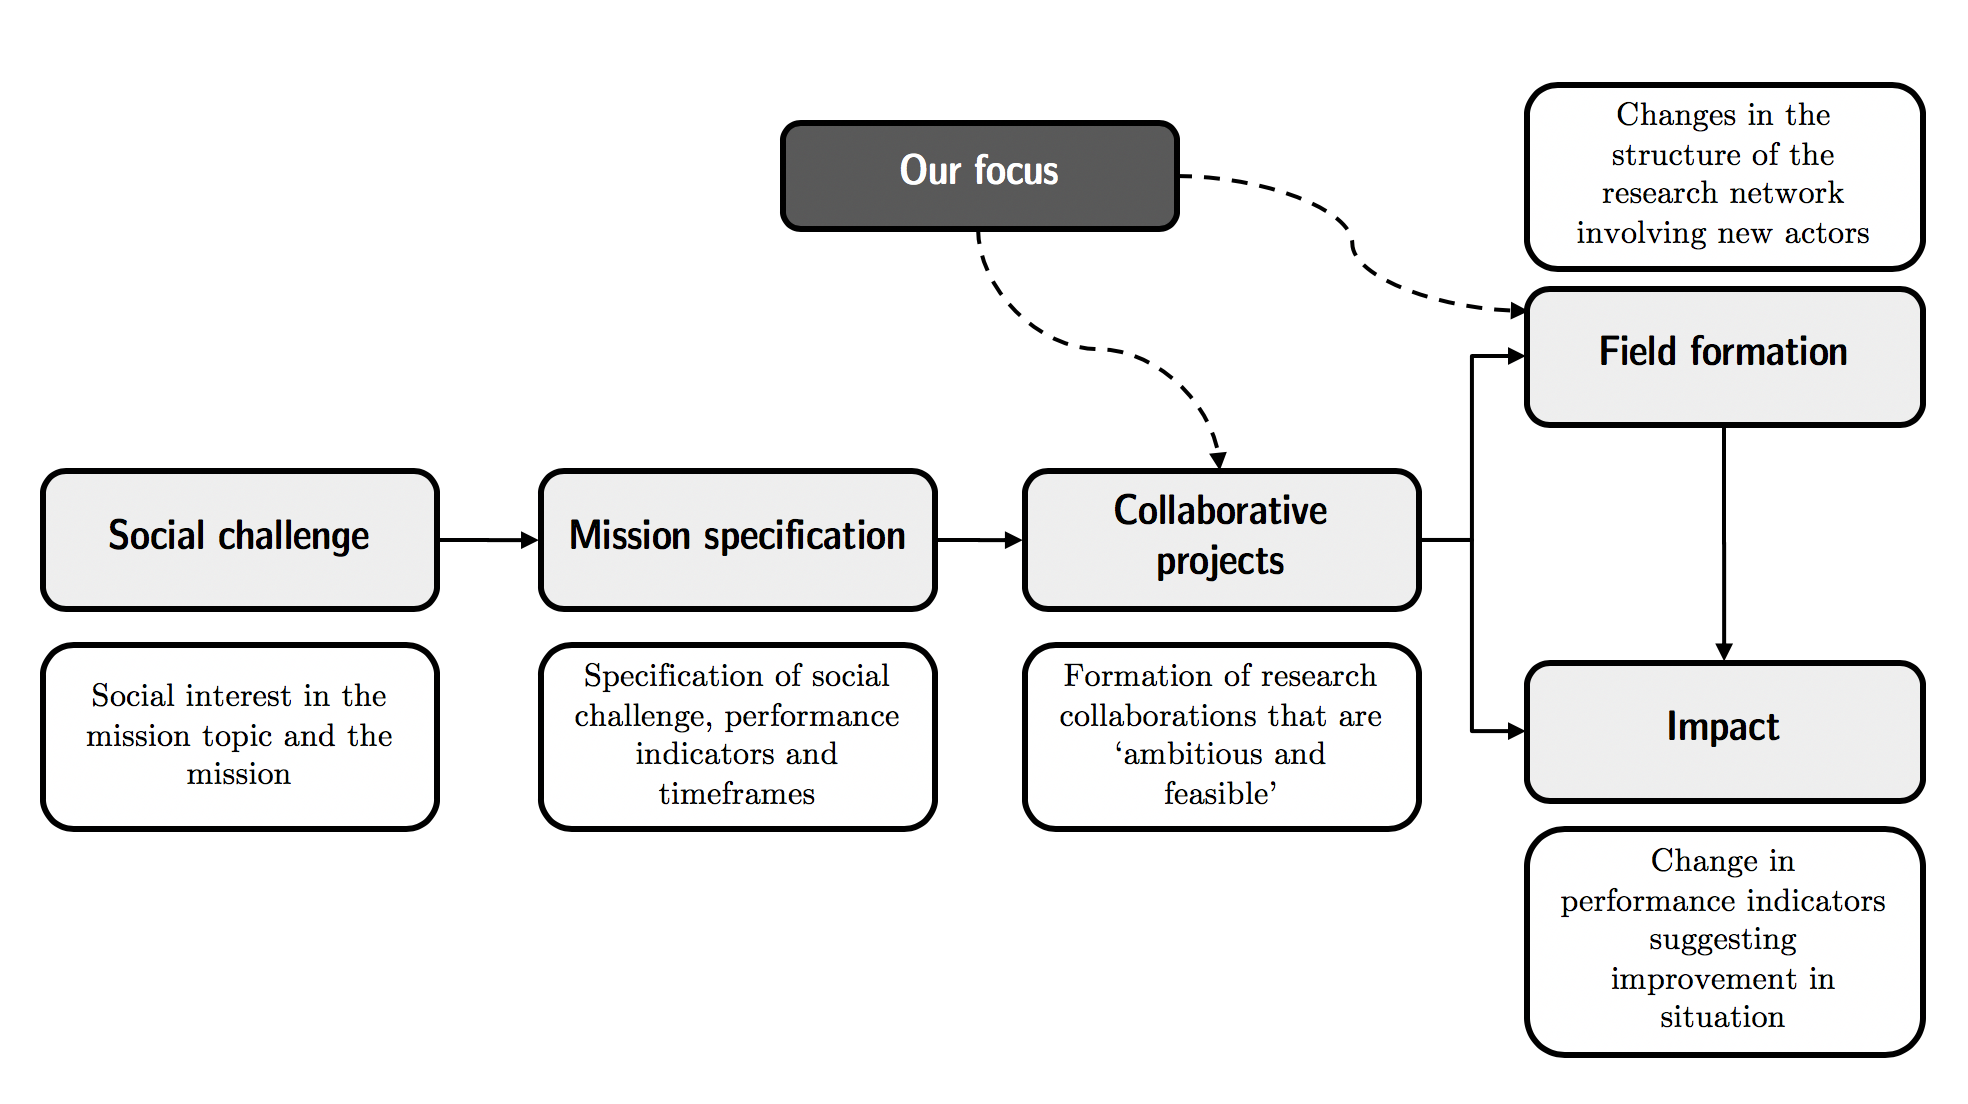
\includegraphics[width=0.9\textwidth]{figures/fig_2_diagram.png}
    \caption{Pathways to impact in a mission, and this paper`s focus}
    \label{fig:diagram}
\end{figure}

It is important to note that the UK Government only announced the Grand Challenge Mission about AI and chronic diseases in 2018. This means that much of our analysis will not capture activities supported by the mission or its impact, but activities already taking place before the mission was launched. In that sense, our analysis should be seen as providing a baseline for the impact of the mission - an important function nevertheless.

\subsection{The mission domain: AI and chronic diseases}
\label{subsec: domain}

Our application domain are research grants in the UK related to the application of Artificial Intelligence (AI) and data to the prevention, diagnosis and treatment of chronic diseases. 

Why is a mission needed in this domain? 

It is widely acknowledged that powerful AI (and machine learning) technologies with strong predictive capabilities could transform how we deal with chronic conditions such as cardiovascular diseases, cancer or diabetes (Cockburn, Henderson, \& Stern, 2018; Loder \& Nicholas, 2018).1 The range of applications is broad, going from identifying the causes of these diseases, to predicting what individuals are at risk, and designing more effective personalised treatments for them (under the rubric of precision medicine). Ultimately, this will contribute to saving lives, improving wellbeing, and lowering costs in healthcare delivery by reducing the need for costly late-treatments (BEIS, 2019).

However, there is a widespread perception that applications of AI in the health domain are lagging behind other application areas such as advertising, social media or finance (J. Mateos-Garcia, 2017; J. C. Mateos-Garcia, 2018; Mulgan, 2017). There are multiple reasons for this including risks of prediction failure, patient data protection and privacy issues, the importance of model explainability and barriers to deployment in large and complex health systems. Overcoming these barriers to the successful deployment of AI in health requires new combinations of knowledge and innovation actors that this mission seeks to encourage.

\subsection{Research questions}
\label{subsec: questions}

Focusing on the UK grand challenge to `Use data, Artificial Intelligence and innovation to transform the prevention, early diagnosis and treatment of chronic diseases by 2030', we will seek to address the following questions:

\begin{enumerate}
    \item What are the levels of activity and funding in this mission field?
    \item How have the levels of activity evolved over time?
    \item What is the disciplinary breakdown of the mission field?
    \item How has the disciplinary breakdown of the mission field evolved over time?
    \item What are the levels of interdisciplinarity in the mission field?
    \item What is the distribution of outcomes in the mission field?
    \item What actors are active in the mission field and what is their `novelty’?
    \item What is the diversity of technological trajectories in the mission field and how it is evolving over time?

\end{enumerate}

\section{Methodology}
\label{sec:methodology}



\subsection{Approach}

Our approach requires two main inputs: a list of keywords describing the contents of a mission (its domain, purpose, technology etc.) and a list of text descriptions about potentially relevant R&I activities to be queried with these keywords. These two inputs are sufficient to map a mission field. Additional metadata such as funding year, level of funding, name of the funder, organisations collaborating in funded projects and outcomes and impacts can be used to  generate additional indicators. 

All this information, is generally available from open datasets about research funding such as the Gateway to Research (which we are using in this paper), the CORDIS database of EU Horizon 2020 funded projects, or the National Institutes of Health World Reporter database of health-related research. It would also be possible to use this approach in other potentially relevant datasets such as patent databases, pre-prints or open source software (with the caveat that they will generally contain a narrow set of disciplines than what is available in broad-based research funding databases). All this means that the approach that we follow in this paper could be applied to other data sources.

In principle, the framework that we develop could also be applied to other missions as long as activities relevant to them are captured in research funding databases, and it is possible to extract keywords from their definition. The facility for this depends on the mission in question. For example, the mission that we selected for this paper has a relatively well defined set of keywords around `AI’ and `chronic conditions’ that can be mapped on the concepts of ‘solution space’ and ‘problem space’. This makes it easier to delineate and analyse the mission field.\footnote{And even in this case there is debate about the definition of what comprises a `chronic condition’, as we will see below.} Other missions, such as the previously mentioned EU mission to reach zero emissions in EU cities by 2030 would require additional background research to identify bodies of research and knowledge that might contribute to achieving the goal in the context of urban infrastructures (the solution space). Of course, the results of the analysis will be sensitive to the keywords that are selected. Our decision to exclude mission impacts from our indicator framework also makes our approach more scalable, since that is one dimension where missions are likely to be highly heterogeneous. One could think of the framework that we present here as a modular component of a broader measurement framework also including indicators of R&I impact that would be specific to the mission under analysis.


\subsection{Data sources}
\label{subsec:data}

The primary source of data that we have used in this paper is UK Research and Innovation’s Gateway to Research (GtR). GtR is an open, linked database with information about all research activities funded by Research Councils and Innovate UK (the UK’s innovation agency), ranging from research grants in academia to innovation vouchers in industry. In January 2019 we queried GtR’s open API and extracted all the information in the database. In total, this includes information about just under 90,000 projects and 38,700 unique organisations.

For each research activity, we potentially have information about its subject and its starting date, the organisations and individual researchers involved, the amounts of funding awarded, and the outputs, including publications, patents, spin-outs and technology outputs (such as software) among others.

Given our reliance on text descriptions to identify relevant projects, and our interest in understanding mission feasibility (which requires information about project outputs which are, for example, not available for Innovate UK projects),
we focus our analysis on the 37,478 grant applications with an informative description in the corpus.\footnote{This involves removing projects with missing and uninformative descriptions such as boilerplate text stating that a project description is not available for confidentiality reasons}. It is also worth noting that GtR only covers research activity systematically since 2006. 98\% of the projects in the data have a starting date in that year or later.

\subsection{Data processing and enrichment}
One area of interest for us is the level of disciplinary and industrial diversity in a mission field. However, projects in GtR are not classified into high-level research disciplines. They are however tagged with a `bottom-up’ taxonomy of 607 research topics. We build a research topic co-occurrence network that we analyse using community detection methods (more specifically, the Louvain algorithm) in order to identify sets of topics that tend to co-occur frequently, representing higher level, latent, disciplines. The communities obtained through this analysis represent seven disciplines: \emph{`arts and humanities'}, \emph{`biological sciences'}, \emph{`engineering and technology'}, \emph{`environmental sciences'}, \emph{`mathematics and computing'}, \emph{`physics' and `social sciences'}.

We use a supervised machine learning approach to classify projects into disciplines, addressing the fact that interdisciplinary projects can belong to more than one discipline. We identify `pure discipline’ projects that only have research topics from one discipline community and combine them into a labelled dataset that we use to train a machine learning model that predicts project discipline labels based on the (pre-processed) text in their abstract.\footnote{82\% of the projects in the data have research topics that belong to a single discipline. Since the Medical Research Council does not use research topics to label its projects, we assume that all the projects it funds are in the Medical Sciences.} We then use this model to predict the discipline mix for all projects in the data. Figure \ref{fig:discipline_classifier} shows model performance.

\footnote{We use grid search over a family of linear models and random forests with different levels of regularisation and leaf sizes, and three-fold cross validation. The best performing classifier is a logistic regression with L2 regularisation and balanced classes.} 

\begin{figure}[!ht]
    \centering
    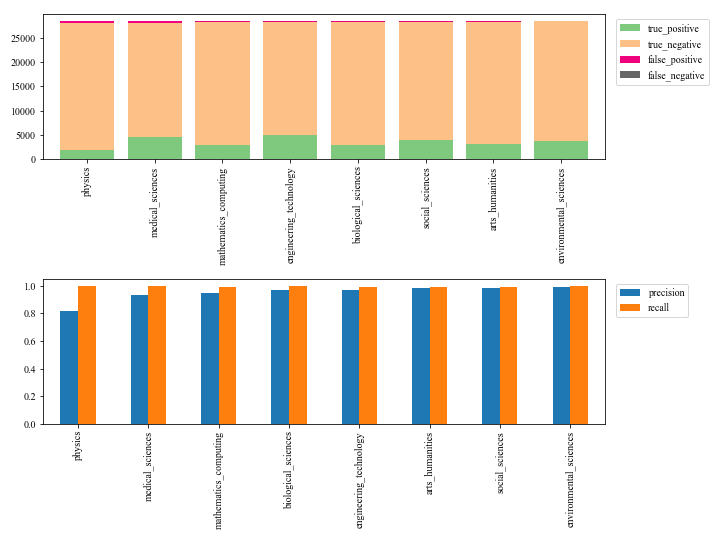
\includegraphics[width=\textwidth]{figures/fig_3_model_validation.png}
    \caption{Figures with the result of the discipline classifier. The top barchart presents a stacked confusion matrix for every discipline representing different classification outcomes, and the bottom barchart presents the precision and recall of every model}
    \label{fig:discipline_classifier}
\end{figure}

Our discipline classifier performs strongly in most cases (the only exception being physics, where the discipline classifier displays lower levels of precision so we exclude it from the rest of our analysis).\footnote{The number of Physics projects in the active mission field was in any case negligible so our results are not affected by this decision.}

\subsection{Operationalising a mission}
In order to answer our research questions, we need to identify projects in the active mission field for the AI and Chronic Diseases mission. To do this, we rely on the mission statement: to \textit{`use data, Artificial Intelligence and innovation to transform the prevention, early
diagnosis and treatment of chronic diseases by 2030'}. 

This mission statement contains the following components:

\begin{enumerate}
    \item \textbf{A subject:} Data, Artificial Intelligence and Innovation
    \item \textbf{A verb:} to Transform
    \item \textbf{An object:} Prevention, early diagnosis and treatment of chronic diseases
    \item \textbf{A timeline:} by 2030
\end{enumerate}

A research project that was completely within the mission would contain all of these elements in its abstract. It is however unlikely that we will find such a match in the data. For instance, few research projects will focus on more than one dimension of the object. Projects will frequently specialise in a single chronic disease or group of chronic diseases. Few projects will specify the dates when they expect to generate applicable findings since that is a policy goal, not a research goal.  We therefore distil the mission statement into the key components that
we would expect to find in a research project abstract. They are the methodology they use (Artificial Intelligence) and their domain (Research on chronic conditions). 

From the point of view of the mission, the methodology is a tool, and the domain is a problem (health challenge) that the methodology seeks to address. Note that we remove from the methodologies terms such as ‘data’ or ‘innovation’ that are rather generic and likely to appear in many irrelevant abstracts. 

Having identified these mission components, we can define a potential mission field and an active mission field. The `potential mission field' comprises all projects that mention at least one mission component - in our case, the tool (AI) or the challenge (chronic diseases). The `active mission field’ comprises the projects that mention all mission components - in our case, the tool and the challenge: these are the most relevant projects from the point of view of the mission (see Figure \ref{fig:venn_diagram} below). One dimension of impact of a mission R\&I policy would be its ability to grow the active mission field at a faster rate that its mission components (reflecting increasing connectivity between them).

\begin{figure}[!ht]
    \centering
    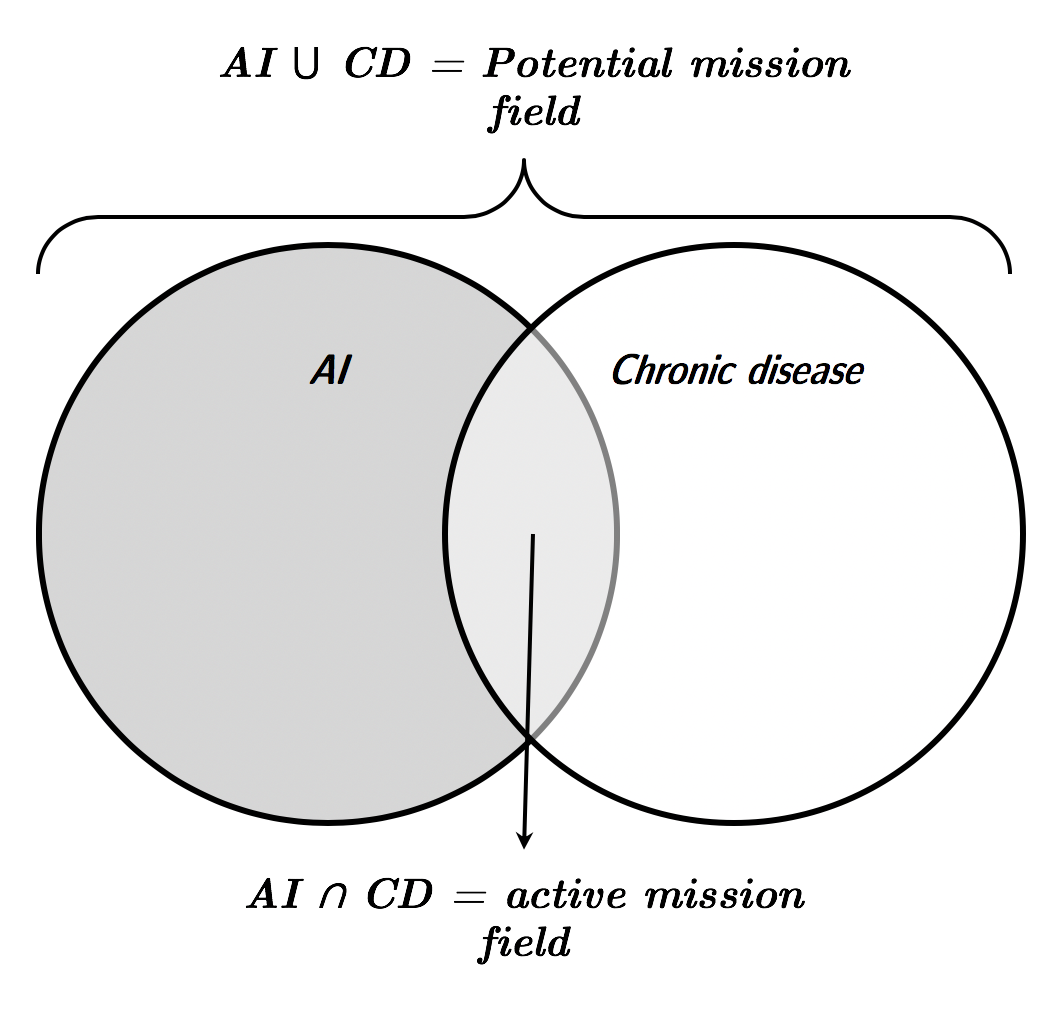
\includegraphics[width=0.7\textwidth]{figures/fig_4_venn.png}
    \caption{Definition of an active mission field and an active mission field}
    \label{fig:venn_diagram}
\end{figure}

\subsection{Definition and expansion of the mission vocabulary}
\label{subsec:vocabulary}

The first step in our analysis is to identify the list of keywords that capture different components of a mission - in our case, AI and chronic diseases. In the case of AI, we use the keyword \emph{artificial intelligence} as well as other related terms such as \emph{machine learning} and specific methodologies and techniques such as \emph{deep learning} or \emph{text mining}.

In the case of chronic diseases, there is no consensus about their definition and the range of diseases and conditions that they include. Given this, we have opted for a crowdsourced list of conditions from wikipedia. This includes the following terms: 

\emph{Addiction, Aids, Alzheimer’s, Atrial fibrillation, Autoimmune disease, Bipolar disorder, Blindness, Cancer, Cardiovascular disease, Cerebral palsy, Chronic condition, Chronic disease, Chronic hepatitis, Chronic pain, Deafness, Depression, Endometriosis, Epilepsy, Hiv, Huntington’s, Hypertension, Lupus, Lymes disease, Parkinsons, Sclerosis, Sickle cell anemia}.

We acknowledge that there is an element of arbitrariness in this definition of chronic diseases. In future applications, the identification of the mission vocabulary should be undertaken in collaboration with the policymakers who defined the mission in order to ensure that the mission field analysis captures the relevant phenomenon.

In order to improve the recall of our queries (that is, our ability to capture relevant entities in the data), we perform a keyword expansion in our original list of terms. This expansion identifies other keywords that are similar to the terms in our original seed list based on their proximity in a word embedding space estimated using the \texttt{Word2Vec} algorithm (Mikolov, Yih, \& Zweig, 2013). This way, we hope to increase the robustness of our results by identifying projects using synonyms of the words included in the initial search.

In order to obtain satisfactory results, we need to tune two parameters in our search algorithm. The first one is the \texttt{window} that \texttt{Word2Vec} considers when identifying the context for a given word (short windows are better for capturing synonyms) and the second is the \texttt{similarity} threshold that we use to identify similar words within the word embedding space. We consider 30 combinations of values for these two parameters and then calculate what is the `model support' for different projects, that is, what proportion of models of classify a project in category (eg AI). 

We split projects into groups based on their rank within the model support distribution and validate a subset of them manually in order to decide a cut-off point in model support. This entails, for every group, checking five projects with a model support above their threshold, and five projects below their threshold. This is the equivalent of checking for true positives (projects that would have been classified in a category eg. AI because they have model support equal above the threshold) and false negatives (projects that would not have been classified in the category because their model support is below the threshold). This leads to select a validation threshold in the seven decile of model support, with a cutoff threshold of $0.46$ (i.e we consider as AI any projects which contains keywords related to AI according to at least 46\% of the \texttt{Word2Vec} models that we trained). At this threshold, our classification of projects into AI had a precision and recall scores of 90\%.\footnote{We classify projects into the chronic disease category if their model support is above 50\%.}

The exhibit next page displays example descriptions of projects that contain both AI and chronic disease keywords. It suggest that even the relatively basic implementation of our vocabulary selection and keyword expansion method yields relevant projects.\footnote{All our code is available in this GitHub repo: \hyperref[https://github.com/Juan-
Mateos/eurito_mission]{https://github.com/Juan-
Mateos/eurito\_mission}. We provide Jupyter Notebooks that describe the steps we have taken in the analysis, and our outputs.}

\begin{tcolorbox}[fontupper=\small, parbox=false]

\textbf{Efficient and Robust Assessment of Cardiovascular Disease Using Machine Learning and Ultrasound Imaging}

ABSTRACT EXCERPT: Heart disease is the number one killer in the world. Currently the best way of diagnosing heart disease and planning its treatment is to use a magnetic resonance imaging (MRI) scanner. However, MRI scanners are expensive and not typically used for scanning hearts in most UK hospitals. Therefore, the best diagnosis and treatment are not available to all patients. Currently the most common way of assessing heart disease is through the use of an ultrasound scanner. Although ultrasound has many advantages, it does not have such good image quality as MRI and so there are difficulties associated with its use in heart disease management. If the 'gold standard' quality of assessment from MRI could somehow be made feasible using ultrasound it would have great potential benefits for patients.

This is the aim of this project. We aim to use state-of-the-art machine learning techniques combined with rich multimodal imaging data to produce a computer model of heart disease and its associations with heart shape and motion. By incorporating MRI as well as ultrasound imaging data into the model we can exploit the power of MRI based only on ultrasound imaging. This would make possible a low cost and easy clinical pathway to the best care possible.

\textbf{Adaptive Automated Scientific Laboratory}
ABSTRACT EXCERPT: Our proposal integrates the scientific method with 21st century automation technology, with the goal of making scientific discovery more efficient (cheaper, faster, better). A Robot Scientist is a physically implemented laboratory automation system that exploits techniques from the field of artificial intelligence to execute cycles of scientific experimentation. Our vision is that within 10 years many scientific discoveries will be made by teams of human and robot scientists, and that such collaborations between human and robot scientists will produce scientific knowledge more efficiently than either could alone. In this way the productivity of science will be increased, leading to societal benefits: better food security, better medicines, etc. The Physics Nobel Laureate Frank Wilczek has predicted that the best scientist in one hundred years time will be a machine. The proposed project aims to take that prediction several steps closer.

We will develop the AdaLab (an Adaptive Automated Scientific Laboratory) framework for semi-automated and automated knowledge discovery by teams of human and robot scientists. This framework will integrate and advance a number of ICT methodologies...

\textbf{Distributed Intelligent Learning Environment for Mammographic Screening}

ABSTRACT EXCERPT: Breast cancer is one of the major causes of death in the modern world. In the UK there is a national screening programme which women between ages of 50 and 70 can attend. Breast cancer screening involves taking breast X-Rays (called mammograms) and examining them for signs of cancer. The idea is that if cancers are detected and treated early (before there are noticeable symptoms) then treatments can be more effective. Examining mammograms for cancer is a highly skilled job carried out by trained radiologists who have to detect what are often very subtle abnormalities occurring only in a small proportion of the cases they examine. Our research will explore how computers can be effectively used to train radiologists to undertake the demanding task of breast screening. To do this we will develop and test an Intelligent Tutoring and e-Learning Environment (ITeLE) to provide instruction, support, practice and feedback for trainee radiologists intending to specialize in mammography...
\end{tcolorbox}

\subsection{Topic modelling}

In Subsection \ref{subsec:trajectory} we want to analyse the thematic composition of the active mission field - that is, what are the topics for research combining AI and chronic diseases in the UK - what applications do they seek to develop, with what goal and in what disease area. This should help us produce indicators about the distribution of activity in the mission field, and whether it is becoming more concentrated or diversified. 

We seek to identify these topics in an automated, unsupervised way using \texttt{TopBSM}, a topic model based on the stochastic block model, a generative model to detect communities in graphs. \texttt{TopSBM} represents corpora of documents containing words as a bipartite graph where words that co-occur in documents are connected in the network, and where documents that share words are also connected. Communities of words in the network represent topics and communities of documents represent segments. Community detection is performed hierarchically making it possible to identify topics (and segments) with different levels of detail. \texttt{TopSBM} has some important advantages over alternative topic modeling algorithms such as Latent Dirichlet allocation: it makes weaker assumptions about the distribution that generates topics in a corpus, and it is able to estimate the number of topics in a document automatically. 

We have trained \texttt{TopSBM} on our grant corpus after pre-processing (including tokenising, removal of rare word and estimation of bigrams and trigrams). Figure depicts the different levels in the hierarchy of our topic model.

\begin{figure}[!ht]
    \centering
    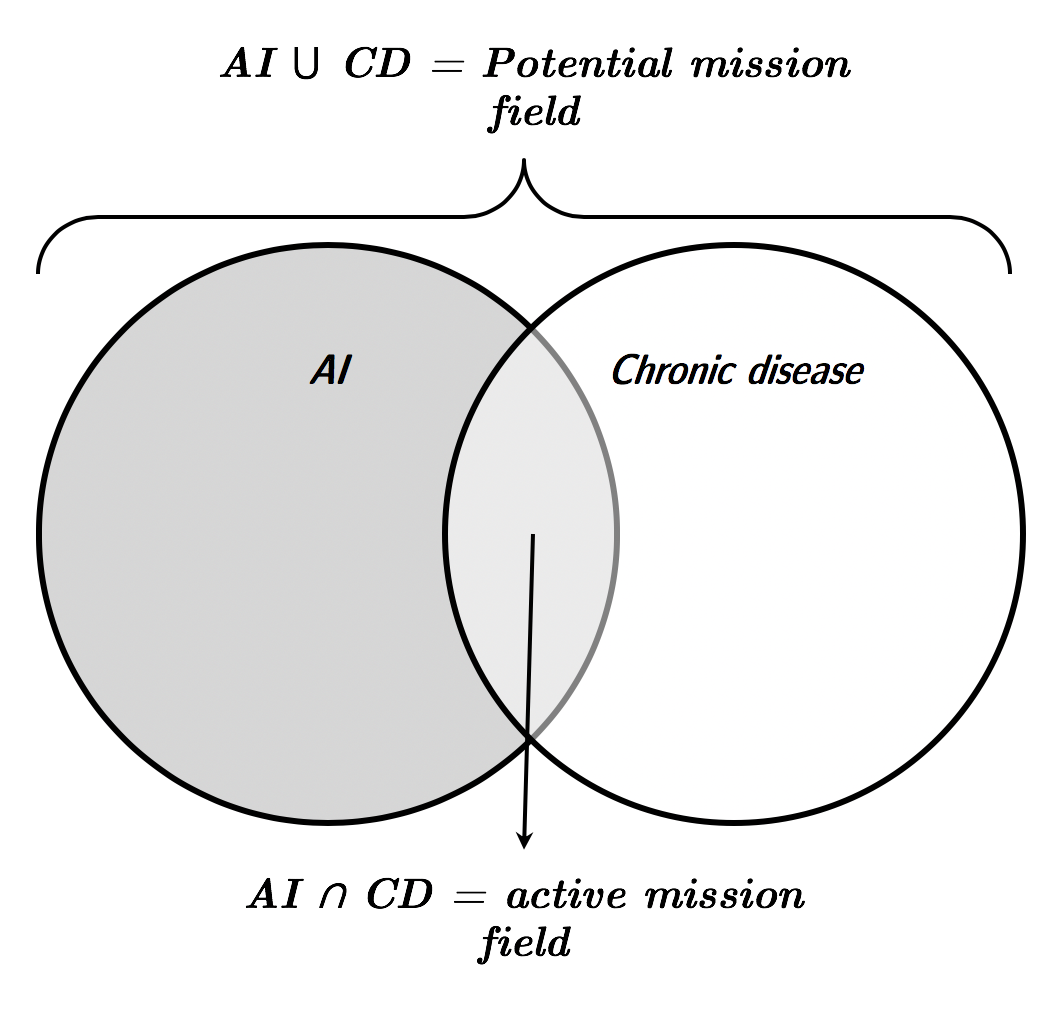
\includegraphics[width=0.7\textwidth]{figures/fig_4_venn.png}
    \caption{Definition of an active mission field and an active mission field}
    \label{fig:venn_diagram}
\end{figure}
 
\section{Findings}
\subsection{Activity and evolution of the mission field}
\subsection{Feasibility}
\subsection{Composition of the mission field}
\subsubsection{Disciplines}
\subsubsection{Actors}
\subsection{Trajectory of the mission field}
\label{subsec:trajectory}
\section{Discussion and conclusions}



\bibliographystyle{apalike}
%\bibliography{aguiar}
%remember to use \citep{} for citation
\end{document}